\documentclass[@BEAMER_OPTIONS@]{beamer}
    @USE_PGFPAGES@

    \usetheme[alternativetitlepage=true,titleline=true]{Torino}
    \setbeamertemplate{navigation symbols}{}
    \setbeamertemplate{note page}[plain]
    \setbeamertemplate{caption}{\insertcaption}

    \usepackage[utf8]{inputenc}
    \usepackage{graphicx}
    \usepackage{subfigure}
    \usepackage{xspace}
    \usepackage{adjustbox}
    \usepackage{tikz}
    \usepgflibrary{arrows}
    \usetikzlibrary{shadows,decorations.pathreplacing,patterns,shapes}
    \tikzstyle{every picture}=[semithick,>=stealth,remember picture]
    \usepackage{listings}
    \lstset{
        language=C++,
        basicstyle=\footnotesize\rmfamily,
        stringstyle=\color{chameleon4},
        numbers=left,
        numberstyle=\tiny,
        aboveskip=-0.02\baselineskip,
        belowskip=-0.02\baselineskip,
        columns=flexible,
        extendedchars=false,
        showstringspaces=false,
        morekeywords={global,kernel,ulong,size_t,get_global_id,get_global_size}
        }
    \newcommand{\code}[1]{\lstinline|#1|}
    \newcommand{\additive}{\hspace{1cm}\footnotesize(\emph{Additive expressions only})}
    \newcommand{\singledevice}{\hspace{1cm}\footnotesize(\emph{Single-device contexts})}
    \newcommand{\plusplus}{{\nolinebreak[4]\hspace{-.05em}\raisebox{.4ex}{\tiny\bf ++}}\xspace}
    \newcommand{\Cpp}{C\plusplus}
    \newcommand{\ghribbon}{
        \begin{tikzpicture}[remember picture,overlay]
            \node[anchor=north east,yshift=4pt,xshift=4pt] at (current page.north east) {
                \href{https://github.com/ddemidov/vexcl}{
\includegraphics[width=2cm]{forkme}}
            };
        \end{tikzpicture}
    }

    \title{VexCL --- a Vector Expression Template Library for OpenCL}

    \author{Denis Demidov}
    \institute{
        Supercomputer Center of Russian Academy of Sciences \\
        Kazan Federal University
    }
    \date{October 2013, Austin, Texas}


\begin{document}

%----------------------------------------------------------------------------
\begin{frame}{}
    \titlepage
\end{frame}

\note{ }

%----------------------------------------------------------------------------
\begin{frame}{Modern GPGPU frameworks}
    \begin{columns}
        \begin{column}{0.45\textwidth}
            \begin{block}{CUDA}
                \begin{itemize}
                    \item Proprietary architecture by NVIDIA
                    \item Requires NVIDIA hardware
                    \item More mature, many libraries
                        \vspace{\baselineskip}
                    \item<2> \emph{Kernels are compiled to PTX together with
                        host program}
                \end{itemize}
            \end{block}
        \end{column}
        \begin{column}{0.45\textwidth}
            \begin{block}{OpenCL}
                \begin{itemize}
                    \item Open standard
                    \item Supports wide range of hardware
                    \item Code is much more verbose
                        \vspace{\baselineskip}
                    \item<2> \emph{Kernels are compiled at runtime, adding an
                        initialization overhead}
                \end{itemize}
            \end{block}
        \end{column}
    \end{columns}
    \vspace{\baselineskip}
    \pause
    \begin{itemize}
        \item The latter distinction is usually considered to be an OpenCL
            drawback.
        \item But it also allows us to generate more efficient kernels at
            runtime!
            \begin{itemize}
                \item VexCL takes care of this part.
            \end{itemize}
    \end{itemize}
\end{frame}

\note[itemize]{
\item Today, major GPGPU programming frameworks are NVIDIA CUDA and OpenCL
\item ...
\item The latter distinction allows one to generate an OpenCL kernel tailored
    for the problem at hand.  And that is what I am going to talk about today.
}

%----------------------------------------------------------------------------
\begin{frame}{VexCL~--- a vector expression template library for OpenCL}
    \ghribbon
    \begin{itemize}
        \item \href{https://github.com/ddemidov/vexcl}{https://github.com/ddemidov/vexcl}
            \vspace{\baselineskip}
        \item Created for ease of \Cpp based OpenCL development.
            \begin{itemize}
                \item Convenient notation for vector expressions.
                \item OpenCL JIT code generation.
            \end{itemize}
        \item The source code is publicly available under MIT license.
            \vspace{\baselineskip}
        \item \emph{This is not a} \Cpp \emph{bindings library!}
            \begin{itemize}
                \item VexCL works on top of Khronos \Cpp bindings for OpenCL.
                \item Easy integration with other libraries or existing
                    projects.
            \end{itemize}
    \end{itemize}
\end{frame}

\note[itemize]{
\item VexCL is a vector expression template library for OpenCL. It uses
    template metaprogramming techniques (in particular, expression templates)
    to provide an intuitive notation for vector and matrix operations.
\item The source code of the library is available on GitHub. It is distributed
    under MIT license, so you are basically free to do whatever you want with
    the library.
\item I would like to note that this is not another C++ bindings library. VexCL
    is designed to work with standard C++ bindings for OpenCL that are provided
    by the Khronos group.
}

%----------------------------------------------------------------------------
\begin{frame}{}
    \tableofcontents[hideallsubsections]
\end{frame}

\note{ }

\section{Motivating example}

\subsection{Hello OpenCL}

%----------------------------------------------------------------------------
\begin{frame}[fragile]{Hello OpenCL: vector sum}
    \begin{block}{Vector sum}
        \begin{itemize}
            \item $A$, $B$, and $C$ are large vectors.
            \item Compute $C = A + B$.
        \end{itemize}
    \end{block}
    \begin{block}{Overview of OpenCL solution}
        \begin{enumerate}
            \item Initialize OpenCL context on supported device.
            \item Allocate memory on the device.
            \item Transfer input data to device.
            \item Run your computations on the device.
            \item Get the results from the device.
        \end{enumerate}
    \end{block}
\end{frame}

\note[itemize]{
\item Let's start with a motivating example. This is classical hello world
    example for OpenCL: addition of two large vector.
\item To do anything with the OpenCL, you need to perform some standard steps,
    like context initialization, memory allocation and transfer, and the
    computations that you needed to do in the first place.
\item So let's look at how these steps are done with native OpenCL API.
}

%----------------------------------------------------------------------------
\begin{frame}[fragile]{Hello OpenCL: vector sum}
    \begin{exampleblock}{1. Query platforms}
        \begin{lstlisting}
std::vector<cl::Platform> platform;
cl::Platform::get(&platform);

if ( platform.empty() )
    throw std::runtime_error("OpenCL platforms not found.");
        \end{lstlisting}
    \end{exampleblock}
\end{frame}

\note[itemize]{
\item First, we need to enumerate OpenCL platforms. Platform is an OpenCL
    implementation by particular provider. Examples are NVIDIA, AMD or Intel
    platforms.
}

%----------------------------------------------------------------------------
\begin{frame}[fragile]{Hello OpenCL: vector sum}
    \begin{exampleblock}{2. Get first available GPU device}
        \begin{lstlisting}[firstnumber=last]
cl::Context context;
std::vector<cl::Device> device;
for(auto p = platform.begin(); device.empty() && p != platform.end(); p++) {
    std::vector<cl::Device> dev;
    try {
        p->getDevices(CL_DEVICE_TYPE_GPU, &dev);
        for(auto d = dev.begin(); device.empty() && d != dev.end(); d++) {
            if (!d->getInfo<CL_DEVICE_AVAILABLE>()) continue;
            device.push_back(*d);
            context = cl::Context(device);
        }
    } catch(...) {
        device.clear();
    }
}
if (device.empty()) throw std::runtime_error("GPUs not found");
        \end{lstlisting}
    \end{exampleblock}
\end{frame}

\note[itemize]{
\item Once we have the list of platforms, we may pick a compute device that
    suites us. In this example we just get first available device that we are
    able to create an OpenCL context on.
}

%----------------------------------------------------------------------------
\begin{frame}[fragile]{Hello OpenCL: vector sum}
    \begin{exampleblock}{3. Create kernel source}
        \begin{lstlisting}[firstnumber=last]
const char source[] =
    "kernel void add(\n"
    "       uint n,\n"
    "       global const float *a,\n"
    "       global const float *b,\n"
    "       global float *c\n"
    "       )\n"
    "{\n"
    "    uint i = get_global_id(0);\n"
    "    if (i < n) {\n"
    "       c[i] = a[i] + b[i];\n"
    "    }\n"
    "}\n";
        \end{lstlisting}
    \end{exampleblock}
\end{frame}

\note[itemize]{
\item Next thing to do is to compile the compute kernels that we will use.
\item With OpenCL, the kernels are compiled at runtime, because OpenCL supports
    wide range of hardware, and each device may have its own set of
    instructions.
\item Here we create string representation of a kernel source.
}

%----------------------------------------------------------------------------
\begin{frame}[fragile]{Hello OpenCL: vector sum}
    \begin{exampleblock}{4. Compile kernel}
        \begin{lstlisting}[firstnumber=last]
cl::Program program(context, cl::Program::Sources(
            1, std::make_pair(source, strlen(source))
            ));
try {
    program.build(device);
} catch (const cl::Error&) {
    std::cerr
        << "OpenCL compilation error" << std::endl
        << program.getBuildInfo<CL_PROGRAM_BUILD_LOG>(device[0])
        << std::endl;
    return 1;
}
cl::Kernel add_kernel = cl::Kernel(program, "add");
        \end{lstlisting}
    \end{exampleblock}
    \begin{exampleblock}{5. Create command queue}
        \begin{lstlisting}[firstnumber=last]
cl::CommandQueue queue(context, device[0]);
        \end{lstlisting}
    \end{exampleblock}
\end{frame}

\note[itemize]{
\item Then we compile an OpenCL program and create a kernel object.
\item We also create the command queue for OpenCL. All OpenCL operations are
    submitted to a command queue. In general, operations submitted to the same
    queue are performed sequentially.
\item And now we are basically done with initialization. All of the above
    operations are usually done once per program lifetime.
}

%----------------------------------------------------------------------------
\begin{frame}[fragile]{Hello OpenCL: vector sum}
    \begin{exampleblock}{6. Prepare input data, transfer it to device}
        \begin{lstlisting}[firstnumber=last]
const size_t N = 1 << 20;
std::vector<float> a(N, 1), b(N, 2), c(N);

cl::Buffer A(context, CL_MEM_READ_ONLY | CL_MEM_COPY_HOST_PTR,
        a.size() * sizeof(float), a.data());

cl::Buffer B(context, CL_MEM_READ_ONLY | CL_MEM_COPY_HOST_PTR,
        b.size() * sizeof(float), b.data());

cl::Buffer C(context, CL_MEM_READ_WRITE,
        c.size() * sizeof(float));
        \end{lstlisting}
    \end{exampleblock}
\end{frame}

\note[itemize]{
\item Next, we need to allocate some device memory and transfer input
    data to the device.
\item The input data is prepared at host in this example. A and B vectors would
    hold ones and twos. This is not very interesting example, but then hello
    world programs never are.
}

%----------------------------------------------------------------------------
\begin{frame}[fragile]{Hello OpenCL: vector sum}
    \begin{exampleblock}{7. Set kernel arguments}
        \begin{lstlisting}[firstnumber=last]
add_kernel.setArg(0, N);
add_kernel.setArg(1, A);
add_kernel.setArg(2, B);
add_kernel.setArg(3, C);
        \end{lstlisting}
    \end{exampleblock}
    \begin{exampleblock}{8. Launch kernel}
        \begin{lstlisting}[firstnumber=last]
queue.enqueueNDRangeKernel(add_kernel, cl::NullRange, N, cl::NullRange);
        \end{lstlisting}
    \end{exampleblock}
    \begin{exampleblock}{9. Get result back to host}
        \begin{lstlisting}[firstnumber=last]
queue.enqueueReadBuffer(C, CL_TRUE, 0, c.size() * sizeof(float), c.data());
std::cout << c[42] << std::endl; // Should get '3' here.
        \end{lstlisting}
    \end{exampleblock}
\end{frame}

\note[itemize]{
\item And now we have everything we need to launch the compute kernel.
\item We set the kernel parameters and submit the kernel to the command queue.
\item Then we transfer the results back to host and see what we got. Here, if
    everything went well, we should get 'three' on standard output.
\item Well, this the ugliest hello world program I ever seen.
\item You will surely agree that a hello world program should fit on one slide.
    And 71 lines of code for a hello world is scary.
\item How much shorter do you think this example will be with VexCL?
}

%----------------------------------------------------------------------------
\begin{frame}[fragile]{Hello VexCL: vector sum}
    \begin{itemize}
        \item Can we use VexCL to achieve same effect with a single slide of
            code?
    \end{itemize}
    \pause
    \begin{exampleblock}{Yes, we can!}
        \begin{lstlisting}
#include <iostream>
#include <vexcl/vexcl.hpp>

int main() {
    std::cout << 3 << std::endl;
}
        \end{lstlisting}
    \end{exampleblock}
\end{frame}

\note{ }

\subsection{Hello VexCL}

%----------------------------------------------------------------------------
\begin{frame}[fragile]{Hello VexCL: vector sum}
    \begin{exampleblock}{Get all available GPUs:}
        \begin{lstlisting}
vex::Context ctx( vex::Filter::Type(CL_DEVICE_TYPE_GPU) );
if ( !ctx ) throw std::runtime_error("GPUs not found");
        \end{lstlisting}
    \end{exampleblock}
    \begin{exampleblock}{Prepare input data, transfer it to device:}
        \begin{lstlisting}[firstnumber=last]
std::vector<float> a(N, 1), b(N, 2), c(N);
vex::vector<float> A(ctx, a);
vex::vector<float> B(ctx, b);
vex::vector<float> C(ctx, N);
        \end{lstlisting}
    \end{exampleblock}
    \begin{exampleblock}{Launch kernel, get result back to host:}
        \begin{lstlisting}[firstnumber=last]
C = A + B;
vex::copy(C, c);
std::cout << c[42] << std::endl;
        \end{lstlisting}
    \end{exampleblock}
\end{frame}

\note[itemize]{
\item Here is the simplest example of using vexcl: addition of two vectors on a
    gpu card.
\item The first line is the context initialization. We provide a device filter
    to the context constructor and get all compute devices that satisfy the
    filter. Here we filter by type and get all available GPUs.
\item Data allocation and transfer is also simplified. \code{vex::vector}
    constructor allocates memory on device and possibly transfers initial data
    as well. The parameters here are list of command queues and either size or
    input host vector.
\item Line ten does what's needs to be done here. This simple expression leads
    to automatic kernel generation and launch. And then we copy the results
    back to host and see what we got.
}

\section{Interface}

%----------------------------------------------------------------------------
\begin{frame}{}
    \tableofcontents[currentsection,hideallsubsections]
\end{frame}

\note{ }

\subsection{Initialization}

%----------------------------------------------------------------------------
\begin{frame}[fragile]{Initialization}
    \begin{itemize}
        \item Multi-device and multi-platform computations are supported.
        \item VexCL context is initialized from combination of device filters.
        \item Device filter is a boolean functor acting on \code{const
            cl::Device&}.
    \end{itemize}
    \vspace{-0.5\baselineskip}
    \begin{overlayarea}{\textwidth}{0.4\textheight}
    \begin{exampleblock}{Initialize VexCL context on selected devices}
        \begin{onlyenv}<1>
        \begin{lstlisting}
vex::Context ctx( vex::Filter::All );
        \end{lstlisting}
        \end{onlyenv}
        \begin{onlyenv}<2|handout:0>
        \begin{lstlisting}
vex::Context ctx( vex::Filter::Type(CL_DEVICE_TYPE_GPU) );
        \end{lstlisting}
        \end{onlyenv}
        \begin{onlyenv}<3|handout:0>
        \begin{lstlisting}
vex::Context ctx(
    vex::Filter::Type(CL_DEVICE_TYPE_GPU) &&
    vex::Filter::Platform("AMD")
    );
        \end{lstlisting}
        \end{onlyenv}
        \begin{onlyenv}<4|handout:0>
        \begin{lstlisting}
vex::Context ctx(
    vex::Filter::Type(CL_DEVICE_TYPE_GPU) &&
    [](const cl::Device &d) {
        return d.getInfo<CL_DEVICE_GLOBAL_MEM_SIZE>() >= 4_GB;
    });
        \end{lstlisting}
        \end{onlyenv}
    \end{exampleblock}
    \end{overlayarea}
    \begin{figure}
        \uncover<1-2,4>{
            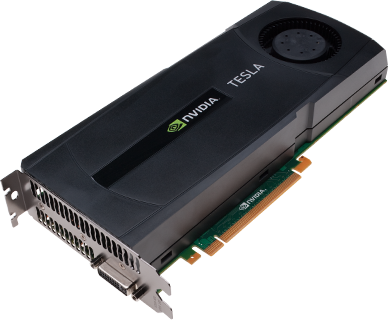
\includegraphics[width=0.2\textwidth]{tesla.png}\quad
        }
        \uncover<1-3>{
            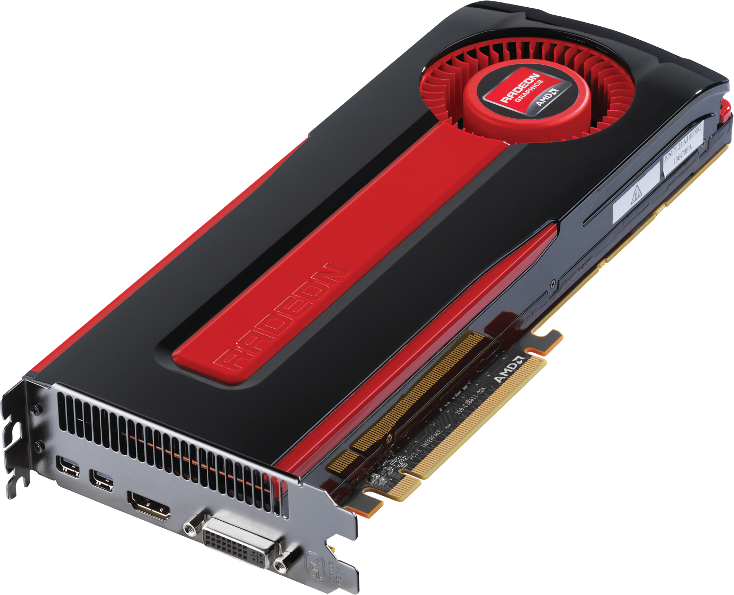
\includegraphics[width=0.2\textwidth]{radeon.png}\quad
        }
        \uncover<1>{
            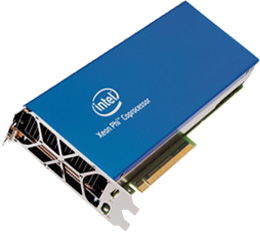
\includegraphics[width=0.16\textwidth]{intel.png}
        }
    \end{figure}
\end{frame}

\note[itemize]{
\item VexCL can transparently work with several compute devices that are
    present on your system.
\item We initialize the VexCL context with a device filter. The device filter
    is a simple functor that acts on cl::Device reference and returns a boolean
    value. Several standard filters are provided and you can write your own
    filters.
\item Let's assume that we have an NVIDIA GPU, an AMD GPU, and an Intel CPU
    installed.
    \begin{enumerate}
        \item The standard 'All' Filter select any device available, so we end
            with three devices in our context.
        \item If we want to select only GPUs, then we can filter the devices by
            type.
        \item It is also possible to combine the device filters with logical
            operators.  Here we select a GPU that is provided by AMD OpenCL
            platform.
        \item And here is an example of a custom filter. Here it selects any
            device that has at least 4GB of memory.
    \end{enumerate}
}

%----------------------------------------------------------------------------
\begin{frame}[fragile]{Exclusive device access}
    \begin{itemize}
        \item \code{vex::Filter::Exclusive()} wraps normal filters to allow
            exclusive access to devices.
            \begin{itemize}
                \item Useful for MPI jobs.
                \item An alternative to NVIDIA's exclusive compute mode for
                    other vendors hardware.
            \end{itemize}
        \item Based on Boost.Interprocess file locks in temp directory.
            \begin{itemize}
                \item Use \code{VEXCL_LOCK_DIR} environment variable to
                    override default behavior.
            \end{itemize}
    \end{itemize}
    \begin{exampleblock}{}
        \begin{lstlisting}
vex::Context ctx( vex::Filter::Exclusive (
    vex::Filter::Env && vex::Filter::Count(1)
    ) );
        \end{lstlisting}
    \end{exampleblock}
    \begin{itemize}
        \item \alert{Only works between programs that actually use the filter.}
    \end{itemize}
\end{frame}

\note[itemize]{
\item Often we want to get an exclusive access to our compute devices. This is
    especially true in a clustered environments, where job manager may tell you
    how many devices are available, but it usually doesn't know which exactly.
\item The Exclusive filter wrapper lets you do this. Internally, lock
    files are created for each compute device present in the system.
\item This obviously will only work between VexCL programs that explicitly ask
    for an exclusive access.
}

\subsection{Memory and work splitting}

%----------------------------------------------------------------------------
\begin{frame}[fragile]{Memory and work splitting}
    \setbeamercovered{transparent=40}
    \begin{exampleblock}{Hello VexCL example}
        \begin{onlyenv}<1|handout:0>
        \begin{lstlisting}[escapechar=!]
vex::Context ctx( vex::Filter::Name("Tesla") );
        \end{lstlisting}
        \end{onlyenv}
        \begin{onlyenv}<2|handout:0>
        \begin{lstlisting}[escapechar=!]
vex::Context ctx( vex::Filter::Type(CL_DEVICE_TYPE_GPU) );
        \end{lstlisting}
        \end{onlyenv}
        \begin{onlyenv}<3>
        \begin{lstlisting}[escapechar=!]
vex::Context ctx( vex::Filter::DoublePrecision );
        \end{lstlisting}
        \end{onlyenv}
        \begin{uncoverenv}<1>
        \begin{lstlisting}[firstnumber=last]

vex::vector<float> A(ctx, N); A = 1;
vex::vector<float> B(ctx, N); B = 2;
vex::vector<float> C(ctx, N);

C = A + B;
        \end{lstlisting}
        \end{uncoverenv}
    \end{exampleblock}
    \setbeamercovered{invisible}
    \begin{figure}
        \begin{tikzpicture}
            \draw (0,3.0) rectangle +(8,0.1);
            \draw (0,3.0) grid[step=0.1] +(8,0.1);
            \draw (-0.3,3.1) node{A};

            \draw (0,2.5) rectangle +(8,0.1);
            \draw (0,2.5) grid[step=0.1] +(8,0.1);
            \draw (-0.3,2.6) node{B};

            \draw (0,2.0) rectangle +(8,0.1);
            \draw (0,2.0) grid[step=0.1] +(8,0.1);
            \draw (-0.3,2.1) node[anchor=center]{C};

            \uncover<1-3> {
            \draw (1,0.5) node{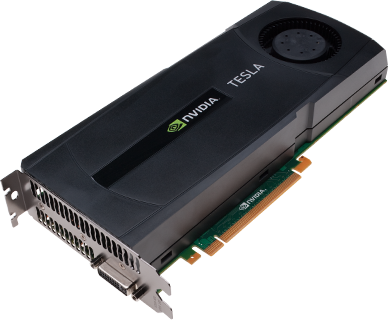
\includegraphics[width=0.2\textwidth]{tesla.png}};
            }

            \uncover<2-3> {
            \draw (4,0.5) node{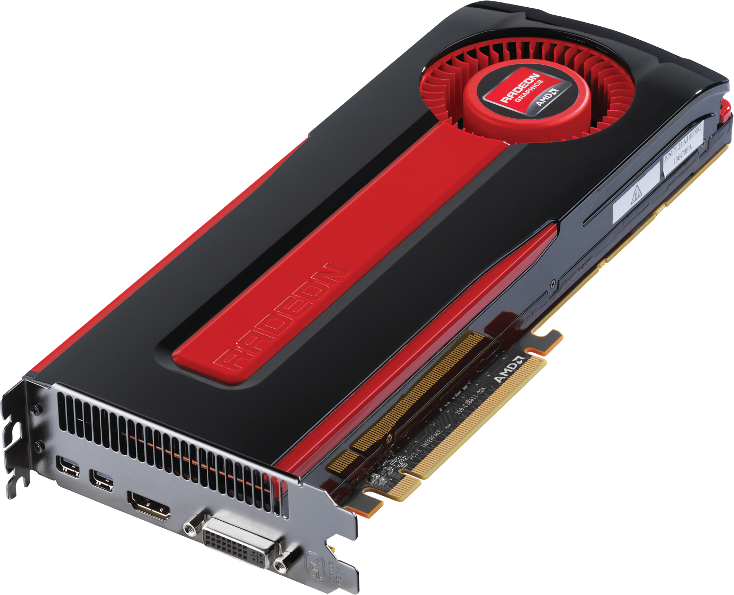
\includegraphics[width=0.2\textwidth]{radeon.png}};
            }

            \uncover<3> {
            \draw (7.5,0.5) node{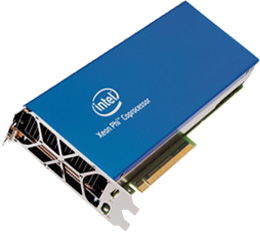
\includegraphics[width=0.16\textwidth]{intel.png}};
            }

            \uncover<1|handout:0> {
            \draw[->,chameleon4,style=dashed] (0,3.2) -- (0,1.8)
                .. controls +(east:0.5) and +(north west:0.5) ..
                (1.4,1.5);
            \draw[->,chameleon4,style=dashed] (8,3.2) -- (8,1.8)
                .. controls +(west:0.5) and +(north east:0.5) ..
                (1.6,1.5);
            }

            \uncover<2|handout:0> {
            \draw[->,chameleon4,style=dashed] (0,3.2) -- (0,1.8)
                .. controls +(east:0.5) and +(north west:0.5) ..
                (1.4,1.5);
            \draw[->,chameleon4,style=dashed] (4,3.2) -- (4,1.8)
                .. controls +(west:0.5) and +(north east:0.5) ..
                (1.6,1.5);

            \draw[->,chameleon4,style=dashed] (4,3.2) -- (4,1.8)
                .. controls +(east:0.1) and +(north west:0.2) ..
                (4.4,1.5);
            \draw[->,chameleon4,style=dashed] (8,3.2) -- (8,1.8)
                .. controls +(west:0.5) and +(north east:0.5) ..
                (4.6,1.5);
            }

            \uncover<3> {
            \draw[->,chameleon4,style=dashed] (0,3.2) -- (0,1.8)
                .. controls +(east:0.5) and +(north west:0.5) ..
                (1.4,1.5);
            \draw[->,chameleon4,style=dashed] (3.5,3.2) -- (3.5,1.8)
                .. controls +(west:0.5) and +(north east:0.5) ..
                (1.6,1.5);

            \draw[->,chameleon4,style=dashed] (3.5,3.2) -- (3.5,1.8)
                .. controls +(east:0.5) and +(north west:0.2) ..
                (4.4,1.5);
            \draw[->,chameleon4,style=dashed] (7,3.2) -- (7,1.8)
                .. controls +(west:0.5) and +(north east:0.5) ..
                (4.6,1.5);

            \draw[->,chameleon4,style=dashed] (7,3.2) -- (7,1.8) -- (7.4,1.5);
            \draw[->,chameleon4,style=dashed] (8,3.2) -- (8,1.8) -- (7.6,1.5);
            }
        \end{tikzpicture}
    \end{figure}
\end{frame}

\note[itemize]{
\item Now that we know how to initialize VexCL context, let's see how device
    vectors are allocated.
\item Here we allocate three vectors, and initialize two of them with
    constant values.
\item Each vector receives a list of queues at initialization.  Since each
    queue corresponds to a specific device, vectors know where to put their
    data to.
    \begin{enumerate}
        \item For example, if we only have the Tesla card in our context, then
            it will hold the complete memory for all of our vectors.
        \item If we use both of the available GPUs, then the vectors will be
            split between the devices. This split is by default proportional to
            the GPU bandwidth and is guaranteed to be consistent for vectors of
            the same size. This consistency allows VexCL to run computations
            independently on all devices in context.
        \item If we add the CPU to the context, it will get smaller share of
            the data and arithmetic operations.
    \end{enumerate}
\item Care must be taken with the use of several devices. VexCL tries to split
    the memory as fair as it can, but it is probable that your program will
    run at the speed of the slowest device.
}

\subsection{Copying memory between host and devices}

%----------------------------------------------------------------------------
\begin{frame}[fragile]{Copies between host and device memory}
    \begin{exampleblock}{}
        \begin{lstlisting}
vex::vector<double> d(ctx, n);
std::vector<double> h(n);
double a[100];
        \end{lstlisting}
    \end{exampleblock}
    \vspace{\baselineskip}
    \begin{columns}
        \begin{column}{0.45\textwidth}
            \begin{exampleblock}{Simple copies}
                \begin{lstlisting}
vex::copy(d, h);
vex::copy(h, d);
                \end{lstlisting}
            \end{exampleblock}
        \end{column}
        \pause
        \begin{column}{0.5\textwidth}
            \begin{exampleblock}{STL-like range copies}
                \begin{lstlisting}
vex::copy(d.begin(), d.end(), h.begin());
vex::copy(d.begin(), d.begin() + 100, a);
                \end{lstlisting}
            \end{exampleblock}
        \end{column}
    \end{columns}
    \vspace{\baselineskip}
    \pause
    \begin{columns}
        \begin{column}{0.45\textwidth}
            \begin{exampleblock}{Map OpenCL buffer to host pointer}
                \begin{lstlisting}
auto p = d.map(devnum);
std::sort(&p[0], &p[d.part_size(devnum)]);
                \end{lstlisting}
            \end{exampleblock}
        \end{column}
        \pause
        \begin{column}{0.5\textwidth}
            \begin{exampleblock}{Inspect or set single element (\emph{slow})}
                \begin{lstlisting}
double v = d[42];
d[0] = 0;
                \end{lstlisting}
            \end{exampleblock}
        \end{column}
    \end{columns}
\end{frame}

\note[itemize]{
\item Copies between host and device memory may be done with simple copy
    function that copy the complete vector either way,
\item or, if you need to do partial copy, you can use STL-like syntax.
\item Vectors also overload array subscript operator, so you can have direct
    read or write access to any element of a vector. But this should be used
    with caution because it is slow. The intended use for this is a single
    element access or debugging.
\item Data may also be accessed through iterators, so it is possible to use,
    for example, an STL algorithm with device vector as a temporary solution.
}


\subsection{Vector expressions}

%----------------------------------------------------------------------------
\begin{frame}[fragile]{What vector expressions are supported?}
    \begin{itemize}
        \item All vectors in an expression have to be \emph{compatible}:
            \begin{itemize}
                \item Have same size
                \item Located on same devices
            \end{itemize}
        \item What may be used:
            \begin{columns}
                \begin{column}{0.42\textwidth}
                    \begin{itemize}
                        \item Vectors and scalars
                        \item Arithmetic, logical operators
                        \item Built-in OpenCL functions
                        \item User-defined functions
                        \item Random number generators
                    \end{itemize}
                \end{column}
                \begin{column}{0.4\textwidth}
                    \begin{itemize}
                        \item Slicing and permutations
                        \item Reduction (sum, min, max)
                        \item Stencil operations
                        \item Sparse matrix~-- vector products
                        \item Fast Fourier Transform
                    \end{itemize}
                \end{column}
            \end{columns}
    \end{itemize}
    \begin{exampleblock}{}
        \begin{lstlisting}
vex::vector<double> x(ctx, n), y(ctx, n);

x = 2 * M_PI * vex::element_index() / n;
y = pow(sin(x), 2.0) + pow(cos(x), 2.0);
        \end{lstlisting}
    \end{exampleblock}
\end{frame}

\note[itemize]{
\item So, what kind of expressions can you use in VexCL?
\item First, any vectors used in an expression have to be compatible.
\item If this requirement is satisfied, then expressions may combine
    vectors and scalars with almost any binary operators. OpenCL math functions
    and user-defined functions are also available.
}

%----------------------------------------------------------------------------
\begin{frame}[fragile]{Builtin operations and functions}
    \begin{columns}
        \begin{column}{0.38\textwidth}
            \begin{exampleblock}{This expression:}
                \begin{lstlisting}
x = 2 * y - sin(z);
                \end{lstlisting}
            \end{exampleblock}
        \end{column}
        \begin{column}{0.55\textwidth}
            \begin{itemize}
                \item Define \code{VEXCL_SHOW_KERNELS} to see the generated code.
            \end{itemize}
        \end{column}
    \end{columns}
    \begin{exampleblock}{\ldots results in this kernel:}
        \begin{lstlisting}
kernel void vexcl_vector_kernel(
    ulong n,
    global double * prm_1,
    int prm_2,
    global double * prm_3,
    global double * prm_4
)
{
    for(size_t idx = get_global_id(0); idx < n; idx += get_global_size(0)) {
        prm_1[idx] = ( ( prm_2 * prm_3[idx] ) - sin( prm_4[idx] ) );
    }
}
        \end{lstlisting}
    \end{exampleblock}
    \begin{tikzpicture}[overlay,scale=0.6]
        \draw (16,8) node(sub)[draw,fill=white,ellipse,drop shadow]{$-$};

        \draw (sub) +(-2.00,-1) node(mul)[draw,fill=white,drop shadow,ellipse]{$*$};
        \draw (sub) +( 2.00,-1) node(sin)[draw,fill=white,drop shadow,ellipse]{sin};
        \draw (mul) +(-2.00,-1) node(two)[draw,fill=white,drop shadow,minimum size=0.5cm]{2};
        \draw (mul) +( 2.00,-1) node(y)  [draw,fill=white,drop shadow,minimum size=0.5cm]{y};
        \draw (sin) +( 1.75,-1) node(z)  [draw,fill=white,drop shadow,minimum size=0.5cm]{z};

        \draw (sub) -- (mul);
        \draw (sub) -- (sin);
        \draw (mul) -- (two);
        \draw (mul) -- (y);
        \draw (sin) -- (z);
    \end{tikzpicture}
\end{frame}

\note{ }

\subsection{Constants}

%----------------------------------------------------------------------------
\begin{frame}[fragile]{Constants}
    \begin{exampleblock}{Macro \code{VEX_CONSTANT} allows to define literal constants}
        \begin{lstlisting}
VEX_CONSTANT(two, 2);
x = two() * y - sin(z);
        \end{lstlisting}
    \end{exampleblock}
    \begin{exampleblock}{}
        \begin{lstlisting}
kernel void vexcl_vector_kernel(
    ulong n,
    global double * prm_1,
    global double * prm_3,
    global double * prm_4
)
{
    for(size_t idx = get_global_id(0); idx < n; idx += get_global_size(0)) {
        prm_1[idx] = ( ( ( 2 ) * prm_3[idx] ) - sin( prm_4[idx] ) );
    }
}
        \end{lstlisting}
    \end{exampleblock}
    \begin{itemize}
        \item Some predefined math constants are available (wrappers to
            \code{boost::math::constants}):
            \begin{itemize}
                \item \code{vex::constants::pi()},
                    \code{vex::constants::root_two()}, etc.
            \end{itemize}
    \end{itemize}
\end{frame}

\subsection{Element indices}

%----------------------------------------------------------------------------
\begin{frame}[fragile]{Element indices}
    \begin{itemize}
        \item \code{vex::element_index(size_t offset = 0)} returns index of an
            element inside a vector.
            \begin{itemize}
                \item The numbering starts with \code{offset} and is continuous
                    across devices.
            \end{itemize}
    \end{itemize}
    \begin{exampleblock}{Linear function:}
        \begin{lstlisting}
vex::vector<double> X(ctx, N);
double x0 = 0, dx = 1e-3;
X = x0 + dx * vex::element_index();
        \end{lstlisting}
    \end{exampleblock}
    \begin{exampleblock}{Single period of sine function:}
        \begin{lstlisting}
X = sin(vex::constants::two_pi() * vex::element_index() / N);
        \end{lstlisting}
    \end{exampleblock}
\end{frame}

\note[itemize]{
\item \code{element_index} is a function that allows you to use element
    position inside of vector expressions.
\item The function may participate in arbitrary vector expressions.
\item For example, here\ldots
}

\subsection{User-defined functions}

%----------------------------------------------------------------------------
\begin{frame}[fragile]{User-defined functions}
    \begin{itemize}
        \item Users may define functions to be used in vector expressions.
        \item There are two options for doing this:
            \begin{itemize}
                \item Provide function body in a string.
                \item Provide generic \Cpp functor.
            \end{itemize}
        \item Once defined, user functions are used in the same way as builtin
            functions.
    \end{itemize}
\end{frame}

\note{ }

%----------------------------------------------------------------------------
\begin{frame}[fragile]{1. Provide function body in a string}
    \begin{itemize}
        \item Choose function name
        \item Specify function signature
        \item Provide function body
    \end{itemize}
    \begin{exampleblock}{Defining a function:}
        \begin{lstlisting}
VEX_FUNCTION( sqr, double(double, double), "return prm1 * prm1 + prm2 * prm2;" );
        \end{lstlisting}
    \end{exampleblock}
    \begin{exampleblock}{Using a function:}
        \begin{lstlisting}
Z = sqrt( sqr(X, Y) );
        \end{lstlisting}
    \end{exampleblock}
\end{frame}

\note[itemize]{
\item It is possible to define an OpenCL function that may be used with vector
    expressions. You need to provide function body, parameter types, and return
    type.
\item Function body has to be of \code{extern const char} type, to allow its
    use as a template parameter. And it has to be defined at global scope.
\item Inside the body function parameters are always named prm1, prm2, etc.
\item Here we define 'between' function that returns true if its second
    parameter is between its first and third parameters. The UserFunction
    object is stateless, so it may be good idea to define it at global scope
    as well, next to its body.
\item Now we may use the function in expressions. Any vector expression may be
    used as a parameter for a user-defined (or builtin) function.
}

%----------------------------------------------------------------------------
\begin{frame}[fragile]{2. Provide generic functor}
    \setbeamercovered{again covered={\opaqueness<1->{40}}}
    \begin{exampleblock}<1,2>{Functor definition:}
        \begin{lstlisting}
struct sqr_functor {
    template <class T>
    T operator(const T &x, const T &y) const {
        return x * x + y * y;
    }
};
        \end{lstlisting}
    \end{exampleblock}
    \pause
    \begin{exampleblock}<2>{Generate VexCL function:}
        \begin{lstlisting}
using vex::generator::make_function;
auto sqr = make_function<double(double,double)>( sqr_functor() );
        \end{lstlisting}
    \end{exampleblock}
    \vspace{0.5\baselineskip}
    \begin{exampleblock}<3>{Boost.Phoenix lambdas \emph{are} generic functors:}
        \begin{lstlisting}
using namespace boost::phoenix::arg_names;
auto sqr = make_function<double(double,double)>( arg1 * arg1 + arg2 * arg2 );
        \end{lstlisting}
    \end{exampleblock}
\end{frame}

\note{ }

%----------------------------------------------------------------------------
\begin{frame}[fragile]{User functions are translated to OpenCL functions}
    \begin{exampleblock}{}
        \begin{lstlisting}
Z = sqrt( sqr(X, Y) );
        \end{lstlisting}
    \end{exampleblock}
    \begin{exampleblock}{\ldots gets translated to:}
        \begin{lstlisting}
double func1(double prm1, double prm2) {
    return prm1 * prm1 + prm2 * prm2;
}

kernel void vexcl_vector_kernel(
    ulong n,
    global double * prm_1,
    global double * prm_2,
    global double * prm_3
)
{
    for(size_t idx = get_global_id(0); idx < n; idx += get_global_size(0)) {
        prm_1[idx] = sqrt( func1( prm_2[idx], prm_3[idx] ) );
    }
}
        \end{lstlisting}
    \end{exampleblock}
    \begin{tikzpicture}[overlay,scale=0.6]
        \draw (16,8.75) node(sqrt)[draw,fill=white,ellipse,drop shadow]{sqrt};

        \draw (sqrt) +(0.00,-2) node(sqr)[draw,fill=white,ellipse,drop shadow]{sqr};

        \draw (sqr) +(-2.00,-1) node(x) [draw,fill=white,drop shadow,minimum size=0.5cm]{x};
        \draw (sqr) +( 2.20,-1) node(y) [draw,fill=white,drop shadow,minimum size=0.5cm]{y};

        \draw (sqrt) -- (sqr);
        \draw (sqr)  -- (x);
        \draw (sqr)  -- (y);
    \end{tikzpicture}
\end{frame}

\note{ }

%----------------------------------------------------------------------------
\begin{frame}[fragile]{Functions may be not only convenient, but also effective}
    \begin{exampleblock}{Same example without using a function:}
        \begin{lstlisting}
Z = sqrt( X * X + Y * Y );
        \end{lstlisting}
    \end{exampleblock}
    \begin{exampleblock}{\ldots gets translated to:}
        \begin{lstlisting}
kernel void vexcl_vector_kernel(
    ulong n,
    global double * prm_1,
    global double * prm_2,
    global double * prm_3,
    global double * prm_4,
    global double * prm_5
)
{
    for(size_t idx = get_global_id(0); idx < n; idx += get_global_size(0)) {
        prm_1[idx] = sqrt( ( ( prm_2[idx] * prm_3[idx] ) + ( prm_4[idx] * prm_5[idx] ) ) );
    }
}
        \end{lstlisting}
    \end{exampleblock}
    \begin{tikzpicture}[overlay,scale=0.6]
        \draw (16,8.75) node(sqrt)[draw,fill=white,ellipse,drop shadow]{sqrt};

        \draw (sqrt) +(0.00,-2) node(sum)[draw,fill=white,ellipse,drop shadow]{$+$};

        \draw (sum) +(-3.00,-1) node(mul1)[draw,fill=white,drop shadow,ellipse]{$*$};
        \draw (sum) +( 3.00,-1) node(mul2)[draw,fill=white,drop shadow,ellipse]{$*$};

        \draw (mul1) +(-2.00,-1) node(x1) [draw,fill=white,drop shadow,minimum size=0.5cm]{x};
        \draw (mul1) +( 2.00,-1) node(x2) [draw,fill=white,drop shadow,minimum size=0.5cm]{x};

        \draw (mul2) +(-2.00,-1) node(y1) [draw,fill=white,drop shadow,minimum size=0.5cm]{y};
        \draw (mul2) +( 2.00,-1) node(y2) [draw,fill=white,drop shadow,minimum size=0.5cm]{y};

        \draw (sqrt) -- (sum);
        \draw (sum)  -- (mul1);
        \draw (sum)  -- (mul2);
        \draw (mul1) -- (x1);
        \draw (mul1) -- (x2);
        \draw (mul2) -- (y1);
        \draw (mul2) -- (y2);
    \end{tikzpicture}
\end{frame}

\note{ }

\subsection{Tagged terminals}

%----------------------------------------------------------------------------
\begin{frame}[fragile]{Tagged terminals}
    \begin{itemize}
        \item Programmer may help VexCL to recognize same terminals by
            tagging them:
    \end{itemize}
    \begin{columns}
        \begin{column}{0.48\textwidth}
            \begin{exampleblock}{Like this:}
                \begin{lstlisting}
using vex::tag;
Z = sqrt(tag<1>(X) * tag<1>(X) +
         tag<2>(Y) * tag<2>(Y));
                \end{lstlisting}
            \end{exampleblock}
        \end{column}
        \begin{column}{0.48\textwidth}
            \begin{exampleblock}{or, equivalently:}
                \begin{lstlisting}
auto x = tag<1>(X);
auto y = tag<2>(Y);
Z = sqrt(x * x + y * y);
                \end{lstlisting}
            \end{exampleblock}
        \end{column}
    \end{columns}
    \begin{exampleblock}{}
        \begin{lstlisting}
kernel void vexcl_vector_kernel(
    ulong n,
    global double * prm_1,
    global double * prm_2,
    global double * prm_3
)
{
    for(size_t idx = get_global_id(0); idx < n; idx += get_global_size(0)) {
        prm_1[idx] = sqrt( ( ( prm_2[idx] * prm_2[idx] ) + ( prm_3[idx] * prm_3[idx] ) ) );
    }
}
        \end{lstlisting}
    \end{exampleblock}
\end{frame}

\note{ }

\subsection{Temporaries}

%----------------------------------------------------------------------------
\begin{frame}[fragile]{Reusing intermediate results}
    \begin{columns}
        \begin{column}{0.48\textwidth}
            \begin{itemize}
                \item Some expressions may have several inclusions of the
                    same subexpression:
            \end{itemize}
            \begin{exampleblock}{}
                \begin{lstlisting}
Z = log(X) * (log(X) + Y);
                \end{lstlisting}
            \end{exampleblock}
            \begin{itemize}
                \item \code{log(X)} will be computed twice here.
                \item One could tag \code{X} and hope that OpenCL compiler is
                    smart enough\ldots
            \end{itemize}
        \end{column}
        \begin{column}{0.48\textwidth}
            \begin{tikzpicture}
                \draw (0,0) node(mul)[draw,fill=white,ellipse,drop shadow,minimum size=0.8cm]{$*$};
                \draw (mul)  +( 1.50,-1) node(sum)  [draw,fill=white,ellipse,drop shadow,minimum size=0.8cm]{$+$};
                \draw (mul)  +(-1.50,-1) node(log1) [draw,fill=chameleon2!50,ellipse,drop shadow,minimum size=0.5cm]{log};
                \draw (sum)  +(-1.50,-1) node(log2) [draw,fill=chameleon2!50,ellipse,drop shadow,minimum size=0.5cm]{log};
                \draw (log1) +( 0.00,-1) node(x1)   [draw,fill=chameleon2!50,drop shadow,minimum size=0.5cm]{x};
                \draw (log2) +( 0.00,-1) node(x2)   [draw,fill=chameleon2!50,drop shadow,minimum size=0.5cm]{x};
                \draw (sum)  +( 1.50,-1) node(y)    [draw,fill=white,drop shadow,minimum size=0.5cm]{y};

                \draw (mul)  -- (log1);
                \draw (mul)  -- (sum);
                \draw (log1) -- (x1);
                \draw (sum)  -- (log2);
                \draw (sum)  -- (y);
                \draw (log2) -- (x2);
            \end{tikzpicture}
        \end{column}
    \end{columns}
\end{frame}

\note{ }

%----------------------------------------------------------------------------
\begin{frame}[fragile]{Temporaries}
    \begin{itemize}
        \item But it is also possible to introduce a temporary variable
            explicitly:
    \end{itemize}
    \begin{exampleblock}{}
        \begin{lstlisting}
auto tmp = vex::make_temp<1>( log(X) );
Z = tmp * (tmp + Y);
        \end{lstlisting}
    \end{exampleblock}
    \begin{exampleblock}{}
        \begin{lstlisting}
kernel void vexcl_vector_kernel(
    ulong n,
    global double * prm_1,
    global double * prm_2,
    global double * prm_3
)
{
    for(size_t idx = get_global_id(0); idx < n; idx += get_global_size(0)) {
        double temp_1 = log( prm_2[idx] );
        prm_1[idx] = ( temp_1 * ( temp_1 + prm_3[idx] ) );
    }
}
        \end{lstlisting}
    \end{exampleblock}
\end{frame}

\note{ }

\subsection{Permutations}

%----------------------------------------------------------------------------
\begin{frame}[fragile]{Permutations \singledevice}
    \begin{itemize}
        \item \code{vex::permutation()} function takes arbitrary (integral
            valued) vector expression and returns permutation functor:
    \end{itemize}
    \pause
    \begin{exampleblock}{Index-based permutation:}
        \begin{lstlisting}
vex::vector<size_t> I(ctx, N);
I = N - 1 - vex::element_index();
auto reverse = vex::permutation(I);
y = reverse(x);
        \end{lstlisting}
    \end{exampleblock}
    \pause
    \begin{exampleblock}{Expression-based permutation:}
        \begin{lstlisting}
auto reverse = vex::permutation(N - 1 - vex::element_index());
y = reverse(x);
        \end{lstlisting}
    \end{exampleblock}
    \pause
    \begin{exampleblock}{Permutations are writable:}
        \begin{lstlisting}
reverse(y) = x;
        \end{lstlisting}
    \end{exampleblock}
\end{frame}

\note{ }

\subsection{Slicing}

%----------------------------------------------------------------------------
\begin{frame}[fragile]{Slicing \singledevice}
    \begin{itemize}
        \item When working with dense multidimensional matrices, it is general
            practice to store those in continuous arrays.
            \begin{itemize}
                \item An instance of \code{vex::slicer<NDIM>} class allows to
                    access sub-blocks of such matrix.
            \end{itemize}
    \end{itemize}
    \begin{exampleblock}{n-by-n matrix and a slicer:}
        \begin{lstlisting}
vex::vector<double> x(ctx, n * n);
vex::slicer<2> slice(vex::extents[n][n]); // Can be used with any vector of appropriate size
        \end{lstlisting}
    \end{exampleblock}
    \pause
    \begin{exampleblock}{Access row or column of the matrix:}
        \begin{lstlisting}[firstnumber=last]
using vex::_;
y = slice[42](x);       // 42nd row
y = slice[_][42](x);    // 42nd column
slice[_][10](x) = y;    // Slices are writable
        \end{lstlisting}
    \end{exampleblock}
    \pause
    \begin{exampleblock}{Use ranges to select sub-blocks:}
        \begin{lstlisting}[firstnumber=last]
using vex::range;
z = slice[range(0, 2, n)][range(10, 20)](x);
        \end{lstlisting}
    \end{exampleblock}
\end{frame}

\note{ }

%----------------------------------------------------------------------------
\begin{frame}[fragile]{Reducing slices \singledevice}
    \begin{itemize}
        \item \code{vex::reduce<RDC>()} function takes multidimensional slice
            of arbitrary expression and reduces it along one or more
            dimensions.
        \item Supported reduction kinds: \code{SUM}, \code{MIN}, \code{MAX}.
    \end{itemize}
    \begin{columns}
        \begin{column}{0.48\textwidth}
            \begin{exampleblock}{Row-wise sum:}
                \begin{lstlisting}
vex::slicer<2> s(extents[n][n]);
y = vex::reduce<vex::SUM>(s[_], x, 1);
                \end{lstlisting}
            \end{exampleblock}
        \end{column}
        \pause
        \begin{column}{0.48\textwidth}
            \begin{exampleblock}{Column-wise maximum absolute value:}
                \begin{lstlisting}
vex::slicer<2> s(extents[n][n]);
y = vex::reduce<vex::MAX>(s[_], fabs(x), 0);
                \end{lstlisting}
            \end{exampleblock}
        \end{column}
    \end{columns}
    \pause
    \vspace{\baselineskip}
    \begin{exampleblock}{The result is vector expression (of reduced size), so
        we may nest reductions:}
        \begin{lstlisting}
vex::vector<double> x(ctx, n * n * n);
vex::vector<double> y(ctx, n);

vex::slicer<3> s3(extents[n][n][n]);
vex::slicer<2> s2(extents[n][n]);

y = reduce<MAX>(s2[_], reduce<SUM>(s3[_], log(x), 2), 1);
        \end{lstlisting}
    \end{exampleblock}
\end{frame}

\note{ }

\subsection{Random number generation}

%----------------------------------------------------------------------------
\begin{frame}[fragile]{Random number generation}
    \begin{itemize}
        \item VexCL provides\footnote{Contributed by
            \href{https://github.com/neapel}{Pascal Germroth}
            $\langle$\href{mailto:pascal@ensieve.org}{pascal@ensieve.org}$\rangle$}
            \emph{counter-based} random number generators from
            Random123\footnote{D E Shaw Research,
                \href{http://www.deshawresearch.com/resources\_random123.html}{http://www.deshawresearch.com/resources\_random123.html}}
            suite.
            \vspace{-0.5\baselineskip}
            \begin{itemize}
                \item The generators are \emph{stateless}; mixing functions are
                    applied to element indices.
                \item Implemented families: \code{threefry} and \code{philox}.
                \item Both pass TestU01/BigCrush; up to \alert{$2^{64}$}
                    independent streams with a period of \alert{$2^{128}$}.
                \item Performance: \alert{$\approx 10^{10}$}~Samples/sec (Tesla
                    K20c).
            \end{itemize}
        \item \code{vex::Random<T,G>}~--- uniform distribution.
        \item \code{vex::RandomNormal<T,G>}~--- normal distribution.
    \end{itemize}
    \vspace{-0.5\baselineskip}
    \begin{exampleblock}{Monte Carlo $\pi$:}
        \begin{lstlisting}
vex::Random<double, vex::random::threefry> rnd;
vex::Reductor<size_t, vex::SUM> sum(ctx);
auto x = vex::make_temp<1>(rnd(vex::element_index(0, n), std::rand()));
auto y = vex::make_temp<2>(rnd(vex::element_index(0, n), std::rand()));
double pi = 4.0 * sum( (x * x + y * y) < 1 ) / n;
        \end{lstlisting}
    \end{exampleblock}
\end{frame}

\note[itemize]{
\item Random number generation is a useful feature that is used often in, e.g.,
    molecular dynamics.
\item Random number generators in VexCL are stateless, so they don't require
    additional storage or global memory interactions. Randomness is obtained by
    applying mixing functions to element indices.
}

\subsection{Reductions}

%----------------------------------------------------------------------------
\begin{frame}[fragile]{Reductions}
    \begin{itemize}
        \item Class \code{vex::Reductor<T, kind>} allows to reduce arbitrary
            \emph{vector expression} to a\\ single value of type \code{T}.
        \item Supported reduction kinds: \code{SUM}, \code{MIN}, \code{MAX}
    \end{itemize}
    \begin{exampleblock}{Inner product}
        \begin{lstlisting}
vex::Reductor<double, vex::SUM> sum(ctx);
double s = sum(x * y);
        \end{lstlisting}
    \end{exampleblock}
    \begin{exampleblock}{Number of elements in x between 0 and 1}
        \begin{lstlisting}
vex::Reductor<size_t, vex::SUM> sum(ctx);
size_t n = sum( (x > 0) && (x < 1) );
        \end{lstlisting}
    \end{exampleblock}
    \begin{exampleblock}{Maximum distance from origin}
        \begin{lstlisting}
vex::Reductor<double, vex::MAX> max(ctx);
double d = max( sqrt(x * x + y * y) );
        \end{lstlisting}
    \end{exampleblock}
\end{frame}

\note[itemize]{
\item Reduction is an operation of reducing a vector to a single value.
\item The most frequent types are summation and finding minimum or maximum
    element of a vector.
\item VexCL provides Reductor functor that accepts any valid vector expression
    as a parameter.
\item For example, to compute an inner product of two vectors we compute sum of
    their elementwise product.
\item To find number of elements in vector x that are greater than zero and
    less than one, we compute sum of the corresponding boolean expression.
\item And to find the maximum distance from axis origin for a set of
    two-dimensional points, we compute exactly that: max of their radius.
}

\subsection{Scattered data interpolation}

%----------------------------------------------------------------------------
\begin{frame}[fragile]{Scattered data interpolation with multilevel B-splines}
    \begin{itemize}
        \item VexCL provides implementation of the MBA algorithm\footnote{
                S. Lee, G. Wolberg, and S. Y. Shin.  Scattered data
                interpolation with multilevel B-Splines.\\ \quad \quad
                \emph{IEEE Trans. Vis. Comput. Graph.}, 3:228–244, 1997.}.
    \end{itemize}
    \vspace{-0.5\baselineskip}
    \begin{columns}
        \begin{column}{0.6\textwidth}
            \begin{itemize}
                \item[]
            \begin{itemize}
                \item The algorithm is initialized with scattered N-dimensional
                    points (stored on host).
                \item Returns approximated value at given coordinates inside
                    vector expression.
            \end{itemize}
            \end{itemize}
            \begin{exampleblock}{}
                \begin{lstlisting}
std::array<double, 2> xmin = {-0.01, -0.01};
std::array<double, 2> xmax = {1.01, 1.01};
std::array<size_t, 2> grid = {5, 5};
std::vector< std::array<double, 2> > coords = {...};
std::vector< double > values = {...};

vex::mba<2> surf(ctx, xmin, xmax, coords, values, grid);
double vol = sum( ds * surf(X, Y) );
                \end{lstlisting}
            \end{exampleblock}
        \end{column}
        \begin{column}{0.333\textwidth}
            \begin{figure}
                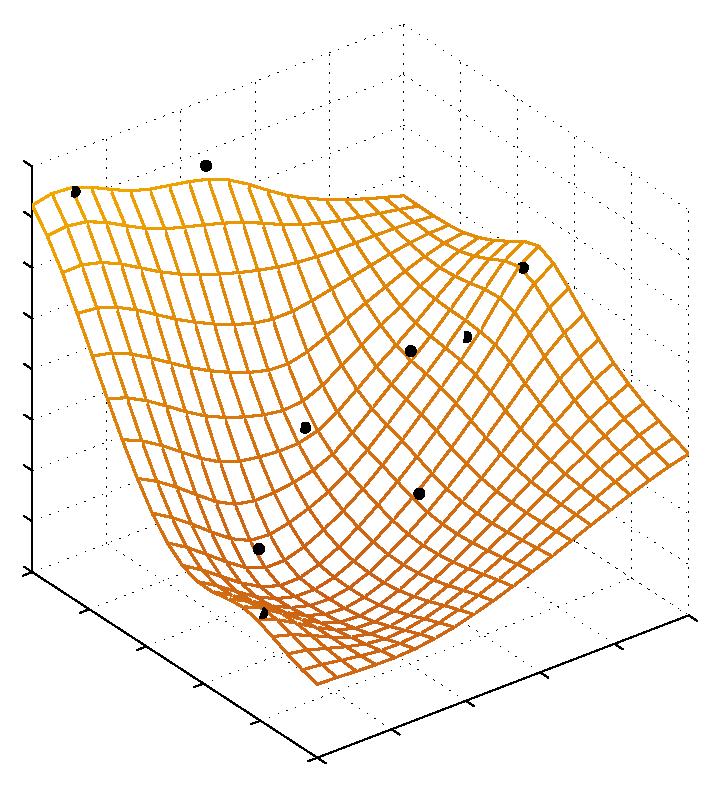
\includegraphics[width=\textwidth]{mba}
            \end{figure}
        \end{column}
    \end{columns}
\end{frame}

\note{ }

\subsection{Sparse matrix~-- vector products}

%----------------------------------------------------------------------------
\begin{frame}[fragile]{Sparse matrix~-- vector products \additive}
    \begin{itemize}
        \item Class \code{vex::SpMat<T>} holds representation of a sparse
            matrix on compute devices.
        \item Constructor accepts matrix in common CRS format:
            \begin{itemize}
                \item row indices, columns and values of nonzero entries.
            \end{itemize}
    \end{itemize}
    \begin{exampleblock}{Construct matrix}
        \begin{lstlisting}
vex::SpMat<double> A(ctx, n, n, row.data(), col.data(), val.data());
        \end{lstlisting}
    \end{exampleblock}

    \begin{exampleblock}{Compute residual value}
        \begin{lstlisting}[firstnumber=last]
// vex::vector<double> u, f, r;
r = f - A * u;
double res = max( fabs(r) );
        \end{lstlisting}
    \end{exampleblock}
\end{frame}

\note[itemize]{
\item Sparse matrix -- vector operation is also provided. A matrix is imported
    from commonly used compressed row storage format.
\item Note that matrix-vector product is not a first-class citizen in vector
    expressions. It uses neighbor values; and neighbors may reside on a
    different compute device. So extra work is needed to exchange data between
    devices. That is why matrix-vector products may only be used in additive
    expressions.
}

%----------------------------------------------------------------------------
\begin{frame}[fragile]{Inlining sparse matrix~-- vector products \singledevice}
    \begin{itemize}
        \item SpMV may only be used in additive expressions:
            \begin{itemize}
                \item Needs data exchange between compute devices.
                \item Impossible to implement with single kernel.
            \end{itemize}
        \item This restriction may be lifted for single-device contexts:
    \end{itemize}
    \begin{exampleblock}{}
        \begin{lstlisting}[numbers=none]
r = f - vex::make_inline(A * u);
double res = max( fabs(r) );
        \end{lstlisting}
    \end{exampleblock}
    \pause
    \begin{exampleblock}{Do not store intermediate results:}
        \begin{lstlisting}[numbers=none]
double res = max( fabs( f - vex::make_inline(A * u) ) );
        \end{lstlisting}
    \end{exampleblock}
\end{frame}

\note{ }

\subsection{Stencil convolutions}

%----------------------------------------------------------------------------
\begin{frame}[fragile]{Simple stencil convolutions \additive}
    \begin{figure}
        \begin{tikzpicture}
            \draw[fill,chameleon4] (2.6,0.6) rectangle +(0.2,0.2);
            \draw[fill,chameleon4] (2.6,0.0) rectangle +(0.2,0.2);

            \draw (0,0) rectangle +(8,0.2);
            \draw (0,0) grid[step=0.2] +(8,0.2);

            \draw (2,0.6) rectangle +(2,0.2);
            \draw (2,0.6) grid[step=0.2] +(2,0.2);

            \draw[chameleon4,decorate,decoration={brace,amplitude=5},yshift=2]
                (2,0.85) -- (4.,0.85);
            \draw (3,1.4) node{width};

            \draw (1.9,0.7) node[anchor=east]{$s$};
            \draw (-0.1,0.1) node[anchor=east]{$x$};
            \draw (4.5,0.6) node[anchor=south west]{$y_i=\sum_k s_k x_{i+k}$};
        \end{tikzpicture}
    \end{figure}
    \begin{itemize}
        \item Simple (linear) stencil is based on a 1D array, and may be used
            e.g. for:
            \begin{itemize}
                \item Signal filters (averaging, low/high pass)
                \item Differential operators with constant coefficients
            \end{itemize}
    \end{itemize}
    \begin{exampleblock}{Moving average with 5-points window:}
        \begin{lstlisting}
std::vector<double> sdata(5, 0.2);
vex::stencil<double> s(ctx, sdata, 2 /* center */);

y = x * s;
        \end{lstlisting}
    \end{exampleblock}
\end{frame}

\note[itemize]{
\item Another commonly used operation is stencil convolution. It may be used to
    filter a one-dimensional signal or to represent a differential operator.
\item A stencil is defined by providing data for its coefficients and
    specifying its center point.
\item To convolve a vector with a stencil you use this simple notation.
\item Stencil convolutions, as well as matrix products, need data from neighbor
    devices; so they may be used only in additive expressions.
}

%----------------------------------------------------------------------------
\begin{frame}[fragile]{User-defined stencil operators \additive}
    \begin{itemize}
        \item Define efficient arbitrary stencil operators:
            \begin{itemize}
                \item Return type
                \item Stencil dimensions (width and center)
                \item Function body
                \item Queue list
            \end{itemize}
    \end{itemize}
    \begin{block}{Example: nonlinear operator}
        \begin{equation*}
            y_i = x_i + \left( x_{i-1} + x_{i+1} \right)^3
        \end{equation*}
    \end{block}
    \begin{exampleblock}{Implementation}
        \begin{lstlisting}
VEX_STENCIL_OPERATOR(custom_op, double, 3/*width*/, 1/*center*/,
    "double t = X[-1] + X[1];\n"
    "return X[0] + t * t * t;",
    ctx);

y = custom_op(x);
        \end{lstlisting}
    \end{exampleblock}
\end{frame}

\note[itemize]{
\item It is also possible to define a custom stencil operation. This may be
    used, for example, if the stencil operator is nonlinear.
\item For this you specify return type, width of the stencil, its center, and
    function body.
\item In the function body you access values through X array. Its elements are
    indexed relatively to the stencil center.
}

\subsection{Raw pointers}

%----------------------------------------------------------------------------
\begin{frame}[fragile]{Raw pointer arithmetic \singledevice}
    \begin{itemize}
        \item \code{raw_pointer(const vector<T>&)} function returns pointer to
            vector's data\\ inside vector expression.
            \begin{itemize}
                \item May be used to implement N-dimensional stencil or
                    N-body problem.
            \end{itemize}
    \end{itemize}
    \begin{exampleblock}{1D Laplace operator:}
        \begin{lstlisting}
VEX_CONSTANT(zero, 0);
VEX_CONSTANT(one,  1);
VEX_CONSTANT(two,  2);

auto ptr   = vex::tag<1>( vex::raw_pointer(x) );

auto i     = vex::make_temp<1>( vex::element_index() );
auto left  = vex::make_temp<2>( if_else(i > zero(),    i - one(), i) );
auto right = vex::make_temp<3>( if_else(i + one() < n, i + one(), i) );

y = *(ptr + i) * two() - *(ptr + left) - *(ptr + right);
        \end{lstlisting}
    \end{exampleblock}
\end{frame}

\note{ }

%----------------------------------------------------------------------------
\begin{frame}[fragile]{Raw pointer arithmetic (Laplace operator)}
    \begin{exampleblock}{}
        \begin{lstlisting}[firstnumber=11]
y = *(ptr + i) * two() - *(ptr + left) - *(ptr + right);
        \end{lstlisting}
    \end{exampleblock}
    \begin{exampleblock}{The generated kernel:}
        \begin{lstlisting}
kernel void vexcl_vector_kernel(
    ulong n,
    global double * prm_1,
    global double * prm_2,
    ulong prm_3,
    ulong prm_4
)
{
    for(size_t idx = get_global_id(0); idx < n; idx += get_global_size(0)) {
        ulong temp_1 = prm_3 + idx;
        ulong temp_2 = temp_1 > 0 ? temp_1 - 1 : temp_1;
        ulong temp_3 = temp_1 + 1 < prm_4 ? temp_1 + 1 : temp_1;
        prm_1[idx] = *(prm_2 + temp_1) * 2 - *(prm_2 + temp_2) - *(prm_2 + temp_3);
    }
}
        \end{lstlisting}
    \end{exampleblock}
\end{frame}

\note{ }

%----------------------------------------------------------------------------
\begin{frame}[fragile]{Raw pointer arithmetic (N-body problem)}
    \begin{equation*}
        y_i = \sum_{j \neq i} e^{-|x_i - x_j|}
    \end{equation*}
    \begin{exampleblock}{}
        \begin{lstlisting}
VEX_FUNCTION(nbody, double(size_t, size_t, double*),
    "double sum = 0, myval = prm3[prm2];\n"
    "for(size_t j = 0; j < prm1; ++j)\n"
    "    if (j != prm2) sum += exp(-fabs(prm3[j] - myval));\n"
    "return sum;\n"
    );

y = nbody(x.size(), vex::element_index(), raw_pointer(x));
        \end{lstlisting}
    \end{exampleblock}
\end{frame}

\note{ }

\subsection{Fast Fourier Transform}

%----------------------------------------------------------------------------
\begin{frame}[fragile]{Fast Fourier Transform \singledevice}
    \begin{itemize}
        \item VexCL provides FFT implementation\footnote{Contributed by
            \href{https://github.com/neapel}{Pascal Germroth}
            $\langle$\href{mailto:pascal@ensieve.org}{pascal@ensieve.org}$\rangle$}:
            \begin{itemize}
                \item Currently only single-device contexts are supported
                \item Arbitrary vector expressions as input
                \item Multidimensional transforms
                \item Arbitrary sizes
            \end{itemize}
    \end{itemize}
    \begin{exampleblock}{Solve Poisson equation with FFT:}
        \begin{lstlisting}
vex::FFT<double, cl_double2> fft(ctx, n);
vex::FFT<cl_double2, double> ifft(ctx, n, vex::inverse);

vex::vector<double> rhs(ctx, n), u(ctx, n), K(ctx, n);
// ... initialize vectors ...

u = ifft( K * fft(rhs) );
        \end{lstlisting}
    \end{exampleblock}
\end{frame}

\note{ }

\subsection{Multivectors \& multiexpressions}

%----------------------------------------------------------------------------
\begin{frame}[fragile]{Multivectors}
    \begin{itemize}
        \item \code{vex::multivector<T,N>} holds \code{N} instances of equally
            sized \code{vex::vector<T>}
        \item Supports all operations that are defined for
            \code{vex::vector<>}.
        \item Transparently dispatches the operations to the underlying
            components.
        \item \code{vex::multivector::operator()(size_t k)} returns \code{k}-th
            component.
    \end{itemize}
    \begin{exampleblock}{}
        \begin{lstlisting}
vex::multivector<double, 2> X(ctx, N), Y(ctx, N);
vex::Reductor<double, vex::SUM> sum(ctx);
vex::SpMat<double> A(ctx, ... );
std::array<double, 2> v;

// ...

X = sin(v * Y + 1);             // X(k) = sin(v[k] * Y(k) + 1);
v = sum( between(0, X, Y) );    // v[k] = sum( between( 0, X(k), Y(k) ) );
X = A * Y;                      // X(k) = A * Y(k);
        \end{lstlisting}
    \end{exampleblock}
\end{frame}

\note[itemize]{
\item This is in principle all of the basic VexCL operations.
\item What is left are multivectors and multiexpressions.
}

%----------------------------------------------------------------------------
\begin{frame}[fragile]{Multiexpressions}
    \begin{itemize}
        \item Sometimes an operation cannot be expressed with simple
            multivector arithmetics.
    \end{itemize}
    \begin{block}{Example: rotate 2D vector by an angle}
        \vspace{-1\baselineskip}
        \begin{align*}
            y_0 &= x_0 \cos \alpha - x_1 \sin \alpha, \\
            y_1 &= x_0 \sin \alpha + x_1 \cos \alpha.
        \end{align*}
    \end{block}

    \begin{itemize}
        \item Multiexpression is a tuple of normal vector expressions
        \item Its assignment to a multivector is functionally equivalent to
            component-wise assignment, but results in a single kernel launch.
    \end{itemize}
\end{frame}

\note[itemize]{
\item Sometimes it's not possible to express the required operation with simple
    multivector arithmetics.
\item For example, take two-dimensional point rotation operation, which is
    defined as this couple of expressions. X and Y coordinates are mixed
    here, so we either have to split the operation in two, or use a
    multiexpression.
}

%----------------------------------------------------------------------------
\begin{frame}[fragile]{Multiexpressions}
    \begin{itemize}
        \item Multiexpressions may be used with multivectors:
    \end{itemize}
    \begin{exampleblock}{}
        \begin{lstlisting}
// double alpha;
// vex::multivector<double,2> X, Y;

Y = std::tie( X(0) * cos(alpha) - X(1) * sin(alpha),
              X(0) * sin(alpha) + X(1) * cos(alpha)  );
        \end{lstlisting}
    \end{exampleblock}
    \begin{itemize}
        \item and with tied vectors:
    \end{itemize}
    \begin{exampleblock}{}
        \begin{lstlisting}
// vex::vector<double> alpha;
// vex::vector<double> odlX, oldY, newX, newY;

vex::tie(newX, newY) = std::tie( oldX * cos(alpha) - oldY * sin(alpha),
                                  oldX * sin(alpha) + oldY * cos(alpha)  );
        \end{lstlisting}
    \end{exampleblock}
\end{frame}

\note[itemize]{
\item You can assign a tuple of expressions to a multivector, or to a tuple of
    single vectors.
\item In either case, this will result in single kernel launch that will update
    all parts of the result at once.
\item Also note that in the second example we rotate every point by its own
    angle stored in alpha vector.
}

%----------------------------------------------------------------------------
\begin{frame}[fragile,shrink=5]{A multiexpression results in a single kernel}
    \begin{exampleblock}{}
        \begin{lstlisting}
auto x0 = tag<0>( X(0) );
auto x1 = tag<1>( X(1) );
auto ca = tag<2>( cos(alpha) );
auto sa = tag<3>( sin(alpha) );

Y = std::tie(x0 * ca - x1 * sa, x0 * sa + x1 * ca);
        \end{lstlisting}
    \end{exampleblock}
    \begin{exampleblock}{}
        \begin{lstlisting}
kernel void vexcl_multivector_kernel(ulong n,
    global double * lhs_1, global double * lhs_2,
    global double * rhs_1, double rhs_2,
    global double * rhs_3, double rhs_4
)
{
    for(size_t idx = get_global_id(0); idx < n; idx += get_global_size(0)) {
        double buf_1 = ( ( rhs_1[idx] * rhs_2 ) - ( rhs_3[idx] * rhs_4 ) );
        double buf_2 = ( ( rhs_1[idx] * rhs_4 ) + ( rhs_3[idx] * rhs_2 ) );

        lhs_1[idx] = buf_1;
        lhs_2[idx] = buf_2;
    }
}

        \end{lstlisting}
    \end{exampleblock}
\end{frame}

\note{ }

%----------------------------------------------------------------------------
\begin{frame}[fragile]{Trick with vex::tie()}
    \begin{itemize}
        \item \code{vex::tie()} returns writable tuple of expressions.
    \end{itemize}
    \begin{exampleblock}{Assign 42 to 5th and 7th rows of x:}
        \begin{lstlisting}
vex::tie( slice[5](x), slice[7](x) ) = 42;
        \end{lstlisting}
    \end{exampleblock}
    \begin{itemize}
        \item It may also be useful for a single expression:
    \end{itemize}
    \begin{exampleblock}{Assign 42 to either y or z depending on value of x:}
        \begin{lstlisting}
vex::tie( *if_else(x < 0, &y, &z) ) = 42;
        \end{lstlisting}
    \end{exampleblock}
\end{frame}

\note{ }

%----------------------------------------------------------------------------
\section{Is it any good?}

\begin{frame}{}
    \tableofcontents[currentsection,hideallsubsections]
\end{frame}

\note{ }

\subsection{Model problem}

%----------------------------------------------------------------------------
\begin{frame}[fragile]{Parameter study for the Lorenz attractor system}
    \begin{columns}
        \begin{column}{0.6\textwidth}
            \begin{block}{Lorenz attractor system}
                \vspace{-1\baselineskip}
                \begin{align*}
                    \dot{x} &= -\sigma \left( x - y \right), \\
                    \dot{y} &= R x - y - xz, \\
                    \dot{z} &= -bz + xy.
                    \label{eq:lorenz}
                \end{align*}
            \end{block}
            \begin{itemize}
                \item Let's solve large number of Lorenz systems, each
                    for a different value of $R$.
                \item Let's use VexCL and Boost.odeint for that.
            \end{itemize}
        \end{column}
        \begin{column}{0.4\textwidth}
            \begin{figure}
                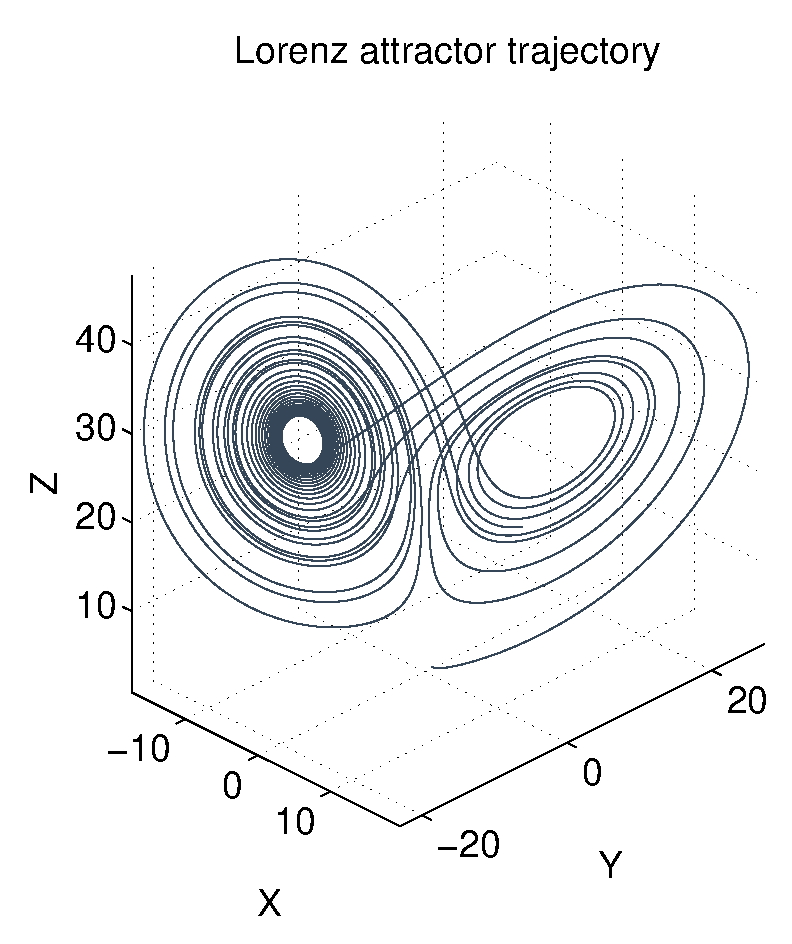
\includegraphics[width=\textwidth]{lorenz}
                \caption{Lorenz attractor trajectory}
            \end{figure}
        \end{column}
    \end{columns}
\end{frame}

\note[itemize]{
\item As an example, lets solve a Lorenz attractor system of ordinary
    differential equations.
\item Lorenz attractor is a particle that moves according to these governing
    equations. The plot on the right shows an example of particle trajectory in
    time.
\item We will solve large number of these Lorenz systems at once.  Each of the
    systems will have its own value for parameter R. That's why this is called
    a parameter study.
}

%----------------------------------------------------------------------------
\begin{frame}{Using Boost.odeint}
    \begin{block}{ODE in general:}
        \begin{equation*}
            \frac{\mbox{d} x}{\mbox{d} t } = \dot{x} = f(x , t),
            \quad \quad x(0) = x_0.
        \end{equation*}
    \end{block}

    \vspace{\baselineskip}

    \begin{exampleblock}{Using Boost.odeint:}
        \begin{enumerate}
            \item Define state type (what is $x$?)
            \item Provide system function (define $f$)
            \item Choose integration method
            \item Integrate over time
        \end{enumerate}
    \end{exampleblock}
\end{frame}

\note[itemize]{
\item Here is a general form of an ODE.
\item In order to use Boost.odeint, one has to...
}

\subsection{Naive implementation}

%----------------------------------------------------------------------------
\begin{frame}[fragile]{Naive implementation}
    \begin{exampleblock}{1. State type}
        \begin{lstlisting}
typedef vex::multivector<double, 3> state_type;
        \end{lstlisting}
    \end{exampleblock}

    \begin{exampleblock}{2. System functor}
        \begin{lstlisting}[firstnumber=last]
struct lorenz_system {
    const vex::vector<double> &R;
    lorenz_system(const vex::vector<double> &R ) : R(R) { }

    void operator()(const state_type &x, state_type &dxdt, double t) {
        dxdt = std::tie( sigma * ( x(1) - x(0) ),
                         R * x(0) - x(1) - x(0) * x(2),
                         x(0) * x(1) - b * x(2)  );
    }
};
        \end{lstlisting}
    \end{exampleblock}
\end{frame}

\note[itemize]{
\item We will hold current state of the system (or set of attractor
    coordinates) in a multivector with 3 components.
\item Here is the definition of the Lorenz system functor: It computes the time
    derivative from current state and time (which is not used here).
\item VexCL make the definition of the functor very simple and intuitive: we
    assign a tuple of vector expressions to the multivector that represents
    time derivative.
}

%----------------------------------------------------------------------------
\begin{frame}[fragile]{Naive implementation}
    \begin{exampleblock}{3. Stepper (4th order Runge-Kutta)}
        \begin{lstlisting}[firstnumber=last]
odeint::runge_kutta4<
        state_type /*state*/,      double /*value*/,
        state_type /*derivative*/, double /*time*/,
        odeint::vector_space_algebra, odeint::default_operations
        > stepper;
        \end{lstlisting}
    \end{exampleblock}
    \begin{exampleblock}{4. Integration}
        \begin{lstlisting}[firstnumber=last]
vex::multivector<double,3> X(ctx, n);
vex::vector<double> R(ctx, n);

X = 10;
R = Rmin + vex::element_index() * ((Rmax - Rmin) / (n - 1));

odeint::integrate_const(stepper, lorenz_system(R), X, 0.0, t_max, dt);
        \end{lstlisting}
    \end{exampleblock}
\end{frame}

\note[itemize]{
\item Next, we create the stepper object and run the integration routine. Here
    we use classic 4th order Runge-Kutta method.
\item And that's it! This was really easy.
\item And, as you will see from the next slide, it was an order of magnitude
    faster than a multithreaded CPU variant.
}

%----------------------------------------------------------------------------
\begin{frame}[fragile]{CUBLAS implementation}
    \begin{itemize}
        \item CUBLAS is a highly optimized BLAS implementation from NVIDIA.
        \item Its disadvantage is that it has fixed number of
            kernels/functions.
        \item Hence, linear combinations (used internally by odeint):
            \begin{equation*}
                x_0 = \alpha_1 x_1 + \alpha_2 x_2 + \cdots + \alpha_n x_n
            \end{equation*}
            are implemented as:
    \end{itemize}
    \begin{exampleblock}{}
        \begin{lstlisting}[numbers=none,texcl=true]
cublasDset(...);        // $x_0 = 0$
cublasDaxpy(...);       // $x_0 = x_0 + \alpha_1 * x_1$
...
cublasDaxpy(...);       // $x_0 = x_0 + \alpha_n * x_n$
        \end{lstlisting}
    \end{exampleblock}
\end{frame}

\note{ }

%----------------------------------------------------------------------------
\begin{frame}[fragile]{Thrust implementation}
    \begin{itemize}
        \item It is possible to fuse linear combination kernels with Thrust:
    \end{itemize}
    \begin{columns}
        \begin{column}{0.70\textwidth}
            \begin{exampleblock}{Thrust}
                \begin{adjustbox}{width=0.95\textwidth,height=0.6\textheight,keepaspectratio}
                    \begin{lstlisting}
struct scale_sum2 {
    const double a1, a2;
    scale_sum2(double a1, double a2) : a1(a1), a2(a2) { }
    template<class Tuple>
    __host__ __device__ void operator()(Tuple t) const {
        thrust::get<0>(t) = a1 * thrust::get<1>(t) + a2 * thrust::get<2>(t);
    }
};

thrust::for_each(
        thrust::make_zip_iterator(
            thrust::make_tuple( x0.begin(), x1.begin(), x2.begin() )
            ),
        thrust::make_zip_iterator(
            thrust::make_tuple( x0.end(), x1.end(), x2.end() )
            ),
        scale_sum2(a1, a2)
        );
                    \end{lstlisting}
                \end{adjustbox}
            \end{exampleblock}
        \end{column}
        \begin{column}<2>{0.22\textwidth}
            \begin{exampleblock}{VexCL}
                \begin{adjustbox}{width=0.95\textwidth,height=0.6\textheight,keepaspectratio}
                    \begin{lstlisting}
x0 = a1 * x1 + a2 * x2;
                    \end{lstlisting}
                \end{adjustbox}
            \end{exampleblock}
        \end{column}
    \end{columns}
\end{frame}

\note{ }

%----------------------------------------------------------------------------
\begin{frame}[fragile]{Performance (Tesla K20c)}
    \begin{figure}
        \only<1|handout:0> {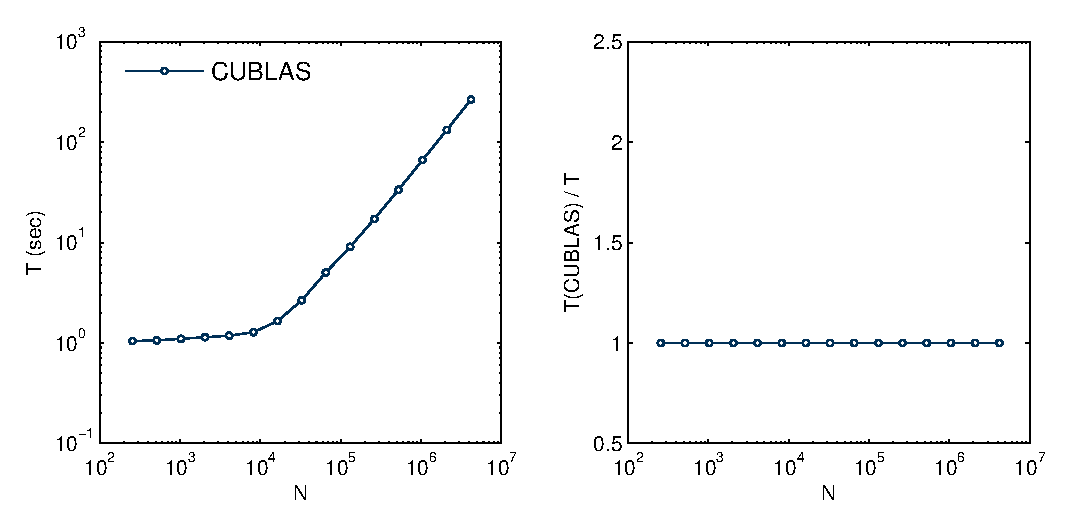
\includegraphics[width=0.9\textwidth]{perfcmp-1}}%
        \only<2|handout:0> {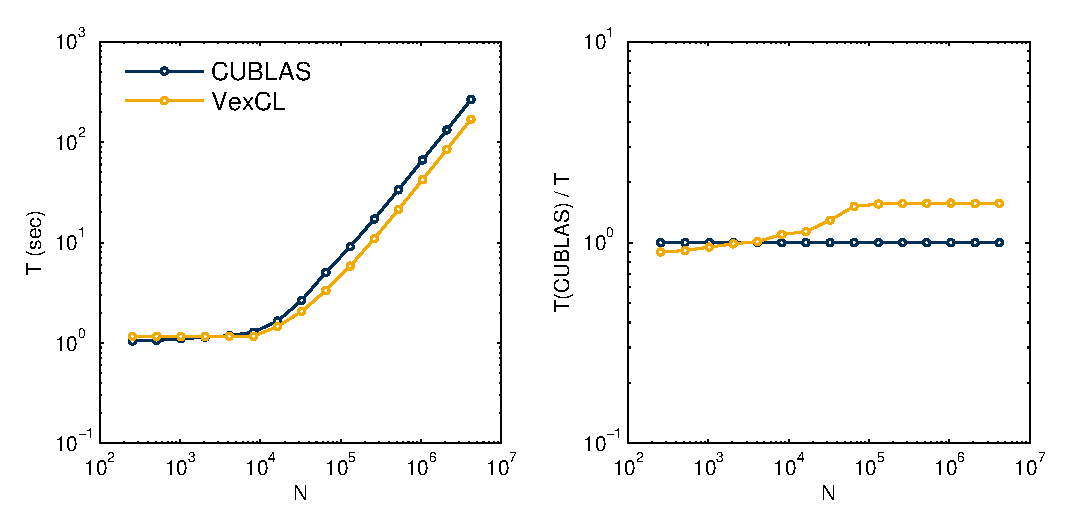
\includegraphics[width=0.9\textwidth]{perfcmp-2}}%
        \only<3|handout:0> {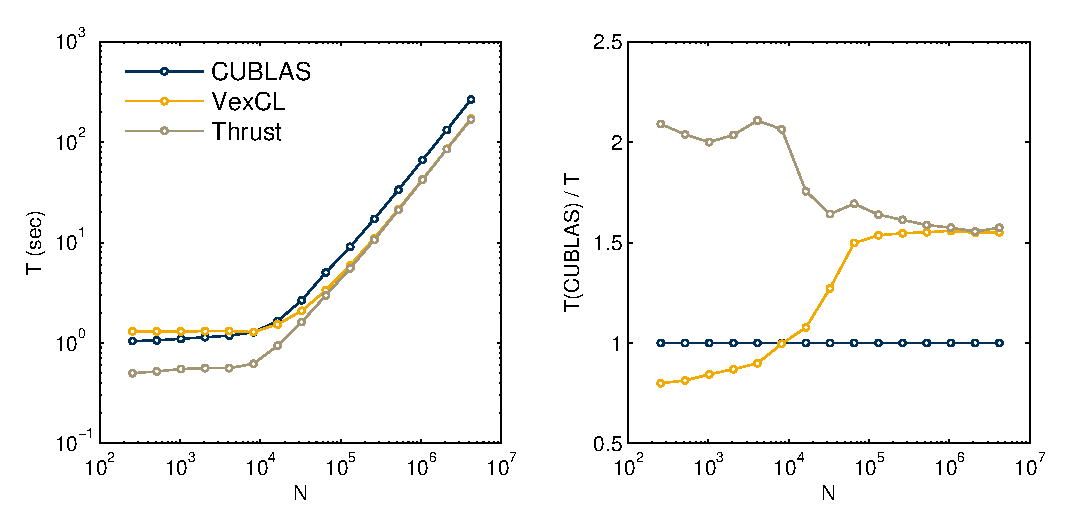
\includegraphics[width=0.9\textwidth]{perfcmp-3}}%
        \only<4->{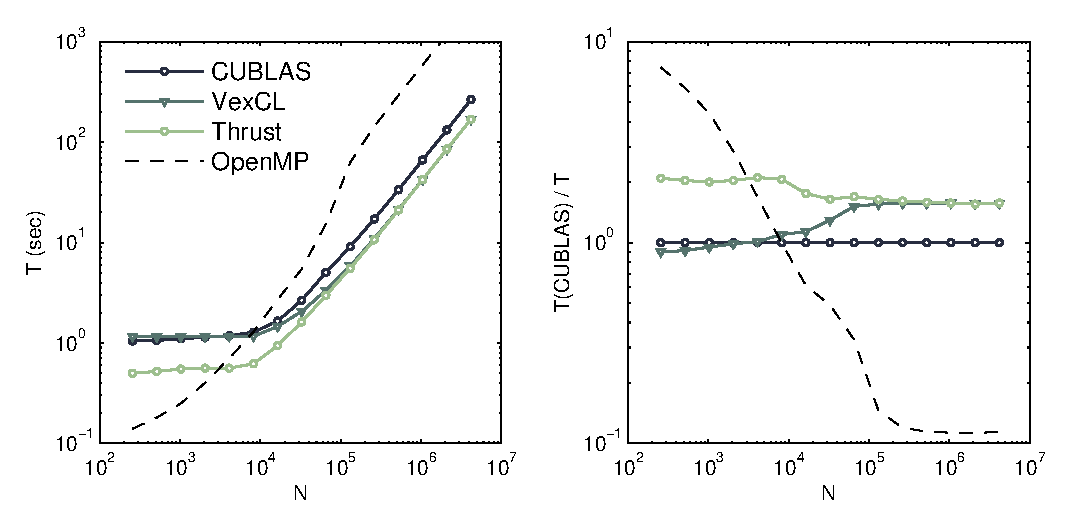
\includegraphics[width=0.9\textwidth]{perfcmp-4}}%
    \end{figure}
    \begin{uncoverenv}<5>
        \begin{itemize}
            \item Deficiencies of naive implementation:
                \begin{itemize}
                    \item Runge-Kutta method uses 4 temporary state variables
                        (here stored on GPU).
                    \item Single Runge-Kutta step results in several kernel
                        launches.
                \end{itemize}
        \end{itemize}
    \end{uncoverenv}
\end{frame}

\note{ }

%----------------------------------------------------------------------------
\begin{frame}[fragile]{What if we did this manually?}
    \begin{columns}
        \begin{column}{0.45\textwidth}
            \begin{itemize}
                \item Create monolithic kernel for a single step of Runge-Kutta
                    method.
                \item Launch the kernel in a loop.
                    \vspace{\baselineskip}
                \item This would be 10x faster!
                    \uncover<2->{\alert{But,}}
                    \begin{itemize}
                        \item<2|alert@2> \emph{We lost odeint's generality.}
                    \end{itemize}
            \end{itemize}
        \end{column} \quad \quad
        \begin{column}{0.5\textwidth}
            \begin{exampleblock}{}
                \begin{adjustbox}{width=0.95\textwidth,height=0.95\textheight,keepaspectratio}
                    \begin{lstlisting}
double3 lorenz_system(double r, double sigma, double b, double3 s) {
    return (double3)( sigma * (s.y - s.x),
                       r * s.x - s.y - s.x * s.z,
                       s.x * s.y - b * s.z);
}
kernel void lorenz_ensemble(
    ulong  n, double dt, double sigma, double b,
    const global double *R,
    global double *X,
    global double *Y,
    global double *Z
    )
{
    for(size_t i = get_global_id(0); i < n; i += get_global_size(0)) {
        double  r = R[i];
        double3 s = (double3)(X[i], Y[i], Z[i]);
        double3 k1, k2, k3, k4;

        k1 = dt * lorenz_system(r, sigma, b, s);
        k2 = dt * lorenz_system(r, sigma, b, s + 0.5 * k1);
        k3 = dt * lorenz_system(r, sigma, b, s + 0.5 * k2);
        k4 = dt * lorenz_system(r, sigma, b, s + k3);

        s += (k1 + 2 * k2 + 2 * k3 + k4) / 6;

        X[i] = s.x; Y[i] = s.y; Z[i] = s.z;
    }
}
                    \end{lstlisting}
                \end{adjustbox}
            \end{exampleblock}
        \end{column}
    \end{columns}
\end{frame}

\note[itemize]{
\item So, what if we did this manually?
\item We would create a single kernel that would do complete Runge-Kutta
    integration step. By the way, here is the kernel that does just that. It's
    very nice-looking kernel in fact.
\item If we run this kernel in a loop, it would give us our solution. And it
    would be ten times faster than our previous variant. So a hundred times
    faster than a CPU! That's an acceleration!
\item But, odeint has 20 different steppers. We don't want to reimplement all
    of those. Let Karsten here do the job, right?
}

\subsection{Kernel generator}

%----------------------------------------------------------------------------
\begin{frame}[fragile]{Convert Boost.odeint stepper to a fused OpenCL kernel!}
    \begin{itemize}
        \item VexCL provides \code{vex::symbolic<T>} type.
        \item An instance of the type dumps any arithmetic operations to output
            stream:
    \end{itemize}
    \begin{exampleblock}{}
        \begin{lstlisting}
vex::symbolic<double> x = 6, y = 7;
x = sin(x * y);
        \end{lstlisting}
    \end{exampleblock}
    \begin{small}
        \begin{verbatim}
double var1 = 6;
double var2 = 7;
var1 = sin( ( var1 * var2 ) );
        \end{verbatim}
    \end{small}
    \pause
    \vspace{-1\baselineskip}
    \begin{itemize}
        \item The idea is very simple:
            \begin{itemize}
                \item Record sequence of arithmetic expressions of an algorithm.
                \item Generate OpenCL kernel from the captured sequence.
            \end{itemize}
    \end{itemize}
\end{frame}

\note[itemize]{
\item VexCL allows to achieve same effect without manual coding.
\item The idea is very simple:
    \begin{itemize}
        \item An algorithm (any algorithm) is just a sequence of arithmetic
            expressions.
        \item VexCL symbolic types allow to record such expressions.
    \end{itemize}
}

%----------------------------------------------------------------------------
\begin{frame}[fragile]{Record operations performed by Boost.odeint stepper}
    \begin{exampleblock}{1. State type}
        \begin{lstlisting}
typedef vex::symbolic< double >   sym_vector;
typedef std::array<sym_vector, 3> sym_state;
        \end{lstlisting}
    \end{exampleblock}

    \begin{exampleblock}{2. System functor}
        \begin{lstlisting}[firstnumber=last]
struct lorenz_system {
    const sym_vector &R;
    lorenz_system(const sym_vector &R) : R(R) {}

    void operator()(const sym_state &x, sym_state &dxdt, double t) const {
        dxdt[0] = sigma * (x[1] - x[0]);
        dxdt[1] = R * x[0] - x[1] - x[0] * x[2];
        dxdt[2] = x[0] * x[1] - b * x[2];
    }
};
        \end{lstlisting}
    \end{exampleblock}
\end{frame}

\note[itemize]{
\item Let's record the sequence of expressions that, for example, Runge-Kutta
    method does, and let's build an OpenCL kernel from this sequence.
\item We replace the state type with array of three symbolic variables. We also
    slightly modify our system functor.
}

%----------------------------------------------------------------------------
\begin{frame}[fragile]{Record operations performed by Boost.odeint stepper}
    \begin{exampleblock}{3. Stepper}
        \begin{lstlisting}[firstnumber=last]
odeint::runge_kutta4<
        sym_state /*state*/,      double /*value*/,
        sym_state /*derivative*/, double /*time*/,
        odeint::range_algebra, odeint::default_operations
        > stepper;
        \end{lstlisting}
    \end{exampleblock}

    \begin{exampleblock}{4. Record one step of Runge-Kutta method}
        \begin{lstlisting}[firstnumber=last]
std::ostringstream lorenz_body;
vex::generator::set_recorder(lorenz_body);

sym_state sym_S = {{ sym_vector(sym_vector::VectorParameter),
                      sym_vector(sym_vector::VectorParameter),
                      sym_vector(sym_vector::VectorParameter) }};
sym_vector sym_R(sym_vector::VectorParameter, sym_vector::Const);

lorenz_system sys(sym_R);
stepper.do_step(std::ref(sys), sym_S, 0, dt);
        \end{lstlisting}
    \end{exampleblock}
\end{frame}

\note[itemize]{
\item We also alter the stepper type accordingly.
\item Next we create the string stream and register it as the expression
    recorder.
\item Finally, we create symbolic variables that would correspond to generated
    kernel parameters, and run single integration step.
\item Now lorenz\_body holds the recorded expression sequence that we
    need.
}

%----------------------------------------------------------------------------
\begin{frame}[fragile]{Generate OpenCL kernel with the recorded sequence}
    \begin{exampleblock}{5. Generate and use OpenCL kernel}
        \begin{lstlisting}[firstnumber=last]
auto lorenz_kernel = vex::generator::build_kernel(ctx, "lorenz", lorenz_body.str(),
        sym_S[0], sym_S[1], sym_S[2], sym_R);

vex::vector<double> X(ctx, n), Y(ctx, n), Z(ctx, n), R(ctx, n);

X = Y = Z = 10;
R = Rmin + (Rmax - Rmin) * vex::element_index() / (n - 1);

for(double t = 0; t < t_max; t += dt) lorenz_kernel(X, Y, Z, R);
        \end{lstlisting}
    \end{exampleblock}
\end{frame}

\note[itemize]{
\item We generate the OpenCL kernel named "lorenz" with the information from
    \code{lorenz_body}. We also supply the symbolic vectors that participated
    in our algorithm. Those will become kernel parameters.
\item Next we create our device vectors, and run the integration loop with the
    generated kernel.
\item And this could be done for any of 20 odeint steppers or for almost any
    other generic algorithm!
}

%----------------------------------------------------------------------------
\begin{frame}{The restrictions}
    \begin{itemize}
        \item Algorithms have to be embarrassingly parallel.
        \item Only linear flow is allowed (no conditionals or data-dependent
            loops).
        \item Some precision may be lost when converting constants to strings.
    \end{itemize}
\end{frame}

\note[itemize]{
\item Of course, there are some restrictions.
}

%----------------------------------------------------------------------------
\begin{frame}[fragile]{Performance of the generated kernel}
    \begin{figure}
        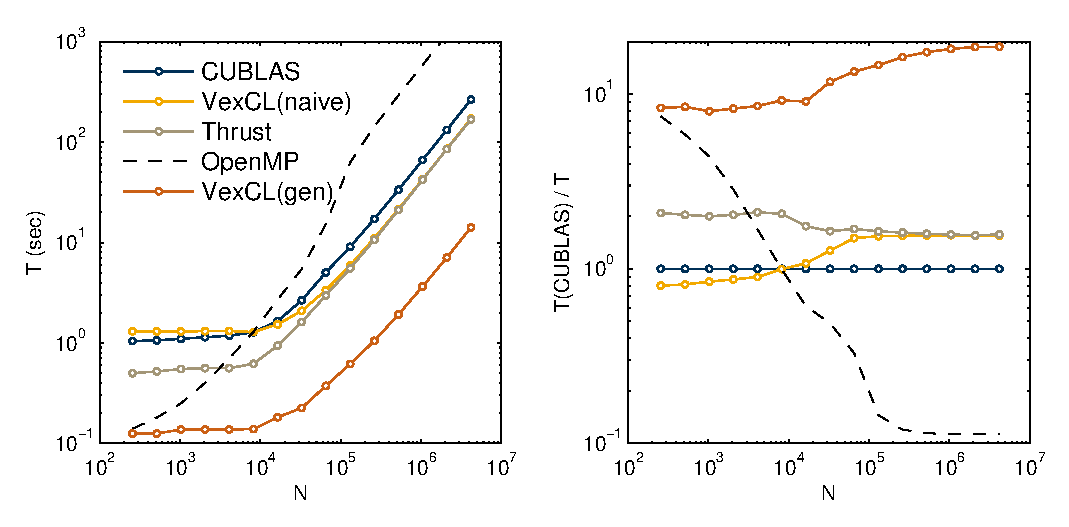
\includegraphics[width=\textwidth]{perfcmp-5}
    \end{figure}
\end{frame}

\note[itemize]{
\item But, as you can see from this slide, the technique allows to achieve same
    acceleration we got from manually coded kernel (Both for CPU and GPU).
}

\section{Summary}

%----------------------------------------------------------------------------
\begin{frame}{Projects already using VexCL}
    \begin{description}[\quad]
        \item[AMGCL] --- implementation of several variants of algebraic
            multigrid:
            \begin{itemize}
                \item \href{https://github.com/ddemidov/amgcl}{https://github.com/ddemidov/amgcl}
            \end{itemize}
            \vspace{\baselineskip}
        \item[Antioch] --- A New Templated Implementation Of Chemistry for
            Hydrodynamics:
            \begin{itemize}
                \item \href{https://github.com/libantioch/antioch}{https://github.com/libantioch/antioch}
            \end{itemize}
            \vspace{\baselineskip}
        \item[Boost.odeint] --- numerical solution of ordinary differential
            equations:
            \begin{itemize}
                \item \href{http://odeint.com}{http://odeint.com}
            \end{itemize}
    \end{description}
    \vspace{\baselineskip}
    \begin{itemize}
        \item \emph{All of these libraries use same generic code for CPU and
            GPU paths}.
    \end{itemize}
\end{frame}

\note{ }



%----------------------------------------------------------------------------
\begin{frame}{Summary}
    \ghribbon
    \begin{itemize}
        \item VexCL allows to write compact and readable code
            without sacrificing performance.
        \item Its code generator allows to convert generic \Cpp
            code to OpenCL at runtime:
            \begin{itemize}
                \item Reduces global memory I/O
                \item Reduces number of kernel launches
                \item Facilitates code reuse
            \end{itemize}
        \item \href{https://github.com/ddemidov/vexcl}{https://github.com/ddemidov/vexcl}
            \vspace{\baselineskip}
        \item Supported compilers (minimal versions; don't forget to enable \Cpp{11} features):
            \begin{itemize}
                \item GCC v4.6
                \item Clang v3.1
            \item MS Visual \Cpp 2010
            \end{itemize}
            \vspace{\baselineskip}
        \item[{[1]}] \href{http://dx.doi.org/10.1137/120903683}{Denis Demidov,
                Karsten Ahnert, Karl Rupp, and Peter Gottschling.\\
                Programming CUDA and OpenCL: A Case Study Using Modern \Cpp
                Libraries.\\
                \emph{SIAM J. Sci. Comput.,} 35(5):C453 – C472, 2013.}
    \end{itemize}
\end{frame}

\note{ }

\end{document}


% vim: et
